In this section the STFT will be implemented and tested to check that it fulfils the test criteria specified in chapter \ref{ch3}. This includes creating a spectrogram from the results of the STFT and check if this is consistent with the expected results.

\subsection{Implementation of the STFT and spectrogram}
The implementation of the STFT requieres an FFT algorithm and will use the algorithm described in algorithm \ref{FFTalg}.
\\ \\
The STFT will be implemented in Python, and the algorithm for the implementation is seen below in algorithm \ref{STFTalg}.
\begin{algorithm}[H]
\caption{STFT algorithm}
\label{STFTalg}
\begin{algorithmic}[1]
\State $FFTsize=1000$ \Comment{Length of window and FFT in STFT}
\State $overlap=2$ \Comment{Number of overlaps of every FFT}
\State $data=$ import of recording \Comment{Recording imported as .wav file}\\
\Procedure{Compute STFT}{}
\State $step=FFTsize/overlap$
\State $w=hanning(FFTsize)$ \Comment{Hanning window of length $=FFTsize$}
\For{each $i$ at intervals of $step$ in length of $data-FFTsize$}
\State $stft = array[FFT(w\cdot data[i:i+FFTsize])]$
\EndFor
\State Return $stft$
\EndProcedure
\end{algorithmic}
\end{algorithm}

The algorithm for generating a spectrogram from the STFT is likewise implemented in Python and is seen in algorithm \ref{SPECTROalg}.
\begin{algorithm}[H]
\caption{Generate spectrogram}
\label{SPECTROalg}
\begin{algorithmic}[1]
\State $freq=$ sampling frequency of data
\State $stft=STFT(data)$ \Comment{Perform STFT on $data$}
\State $time=len(data)/freq$ \Comment{Length of data in seconds.}
\State $stft=20\cdot log_{10}(abs(stft.T))$ \Comment{dB gain of transposed $stft$}\\
\State $x=linspace(0,tid,len(X[1]))$ \Comment{Ticks for x-axis}
\State $y=linspace(0,freq/2,len(len(X[0])$ \Comment{Ticks for y-axis}\\
\State $spec=pcolormesh(x,y,X)$ \Comment{Plot amplitudes as colors with positions $(x,y)$}
\State $colorbar(spec)$ \Comment{Legend of colors illustrated as a colorbar}
\end{algorithmic}
\end{algorithm}

\subsection{Validation of the STFT and spectogram}
The validation of the STFT and spectrograms will be done as a whole entity, and the test specification consists of generating a spectrogram from a signal containing a single sinusoidal wave, which changes frequency once during the sampling interval. The signal is defined as
\begin{align}\label{eq:SPECTROsignal}
sig(x)=\begin{cases}\sin(2\pi x)\,\text{for }x<\frac{t}{2}\\
\sin(6\pi x)\,\text{for }x\geq\frac{t}{2}
\end{cases}.
\end{align}

The sine waves are then with frequencies of 1 and 3 Hz, respectively, and the signal is sampled for $t=26214$ seconds at $f_s=10$ Hz. Figure \ref{fig:test_stft} shows spectrograms of the signal generated with windows of different lengths.
\begin{figure}[H]
\centering
\begin{subfigure}{0.49\textwidth}
\centering
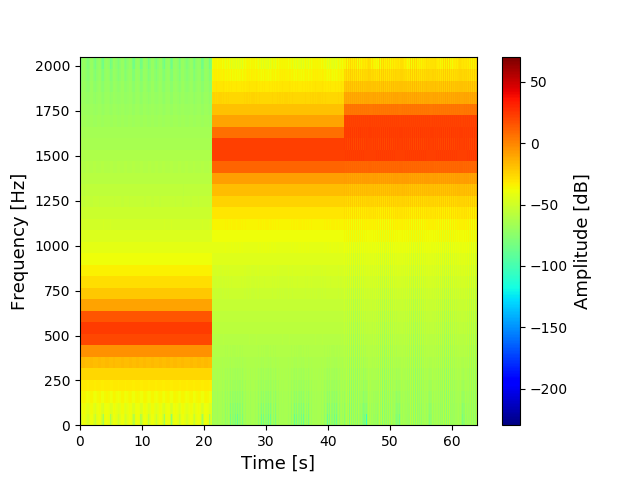
\includegraphics[width=0.9\textwidth]{figures/validation/stft/1.png}
\caption{Spectrogram of signal in \eqref{eq:SPECTROsignal} generated with window of length 100 and overlap of 2. The clear transition from one frequency to another in time and the low resolution in frequency follow from a narrow window used in the STFT.}
\label{fig:test_stft1}
\end{subfigure}
\begin{subfigure}{0.49\textwidth}
\centering
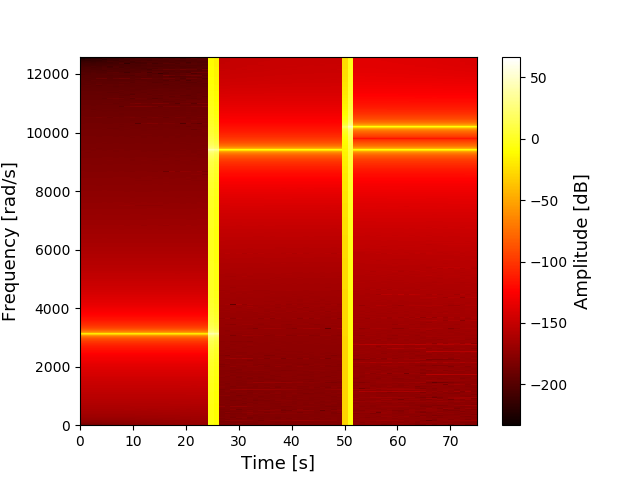
\includegraphics[width=0.9\textwidth]{figures/validation/stft/2.png}
\caption{Spectrogram of signal in \eqref{eq:SPECTROsignal} generated with window of length 10000 and overlap of 2. The clearly visible frequencies in the signal and bad transition from one frequency to another in time follows from a wide window used in the STFT.}
\label{fig:test_stft2}
\end{subfigure}
\caption{Spectrograms of the signal in \eqref{eq:SPECTROsignal} with a narrow and wide window, respectively.}
\label{fig:test_stft}
\end{figure}

From figure \ref{fig:test_stft} it is clearly seen how the length of the window in the STFT used for generating the spectrogram affects the resolution in time and frequency. This agrees with Heisenberg's uncertanity principle described in section \ref{sec:heisenberg}, and so there must be made a tradeoff between the two resolutions. For the purpose of this project it is decided, that...\frede{Her skal vi lige blive enige om hvad vi gør med opløsningen.}
\\ \\
It is therefore concluded that the implementation of the STFT and spectrogram work as intended.